\chapter{Natural Language Processing}
\label{chap:nlp}

It is often challenging to realize the complexity behind \glsfirst{nl}, even to experts. First of all, Language is an academic field of study, implying multi-disciplinary skills. And secondly, staying up to date with evergrowing tools and new \gls{sota} algorithms proves to be challenging. \gls{nl} is the fundamental communication element for humans, \gls{nlp} is the field of \gls{ml} studying \gls{nl} with the goal of providing the ability to machines to handle and mimic \gls{nl} to create human-like verbal interactions. Beyond words and grammar rules, \gls{nl} is a complex orchestration of subtleties, intuitively handled by humans, but not for easily handled by machines. Nonetheless, \glspl{nlp} technologies are massively used in our daily lives, including information extraction, summarization, and conversation simulation. However, even if machines are given the same language rules as humans, they do not yet understand the manipulation they are processing, as humans would do. Indeed, \gls{nlp} algorithms are applying pre-defined or multiple examples-based learned rules, which may result in ambiguities while applying \gls{nl}. Using a rule-based approach \ref{chatbot:rulebased} to build a \gls{nl} model would result into near to infinite amount of conditions, this is the main reason for \gls{nlp} to be particularly present \gls{ml}, particularly in \gls{dl}. 


%\section{\acrlong{nlp} Technologies}
\section{Word Embeddings}
\label{nlp:we}
Commonly used as the first data pre-processing in \gls{dl} \gls{nlp}. Those \glsfirst{ul} algorithms capture syntactical and semantical words representation from large unlabelled corpora datasets as vectors by building a multi-dimensional matrix. On average, dimensions are held in a scope of 100 to 400, and thanks to its the vectorized nature captured words, geometrical operations can be applied, such as the cosine functions to calculate word similarities. Another feature related to word embeddings, is the ability to apply analogical operations such as \textit{'king' - 'man' + 'woman' = 'queen'}, which popularize Word2Vec \ref{nlp:word2vec} and gave credits to the method, even if the justification to this effect has been theorietized 4 years later \footnote{Skip-Gram - Zipf + Uniform = Vector Additivity \autocite{paper:gittens-etal-2017-skip}} by stating that the compositionality is only seen when assumptions are held, in particular when words are uniformly distributed in the embedding space.

\subsection{Word2Vec and GloVe}
\label{nlp:word2vec}
Published by \textit{Google} in 2013, Word2Vec \autocite{paper:word2vec}, and its competitor GloVe \autocite{paper:glove} published by the \textit{University of Standford} in 2014, both use a \gls{snn}, as illustrated on Figure ~\ref{fig:fig_snn}, similarly to \gls{sl} by feeding as input a text corpora, and outputting word vectors with a given vocabulary. Training and testing is straightforward but painful tweaking make it hard to build good generalized word embedding representations. Even if the \gls{snn} could remind a \gls{dl} approach, it is only has one hidden layer; however, the output word vectors are particularly useful for \gls{dnn} as input.

\begin{figure}
    \centering
    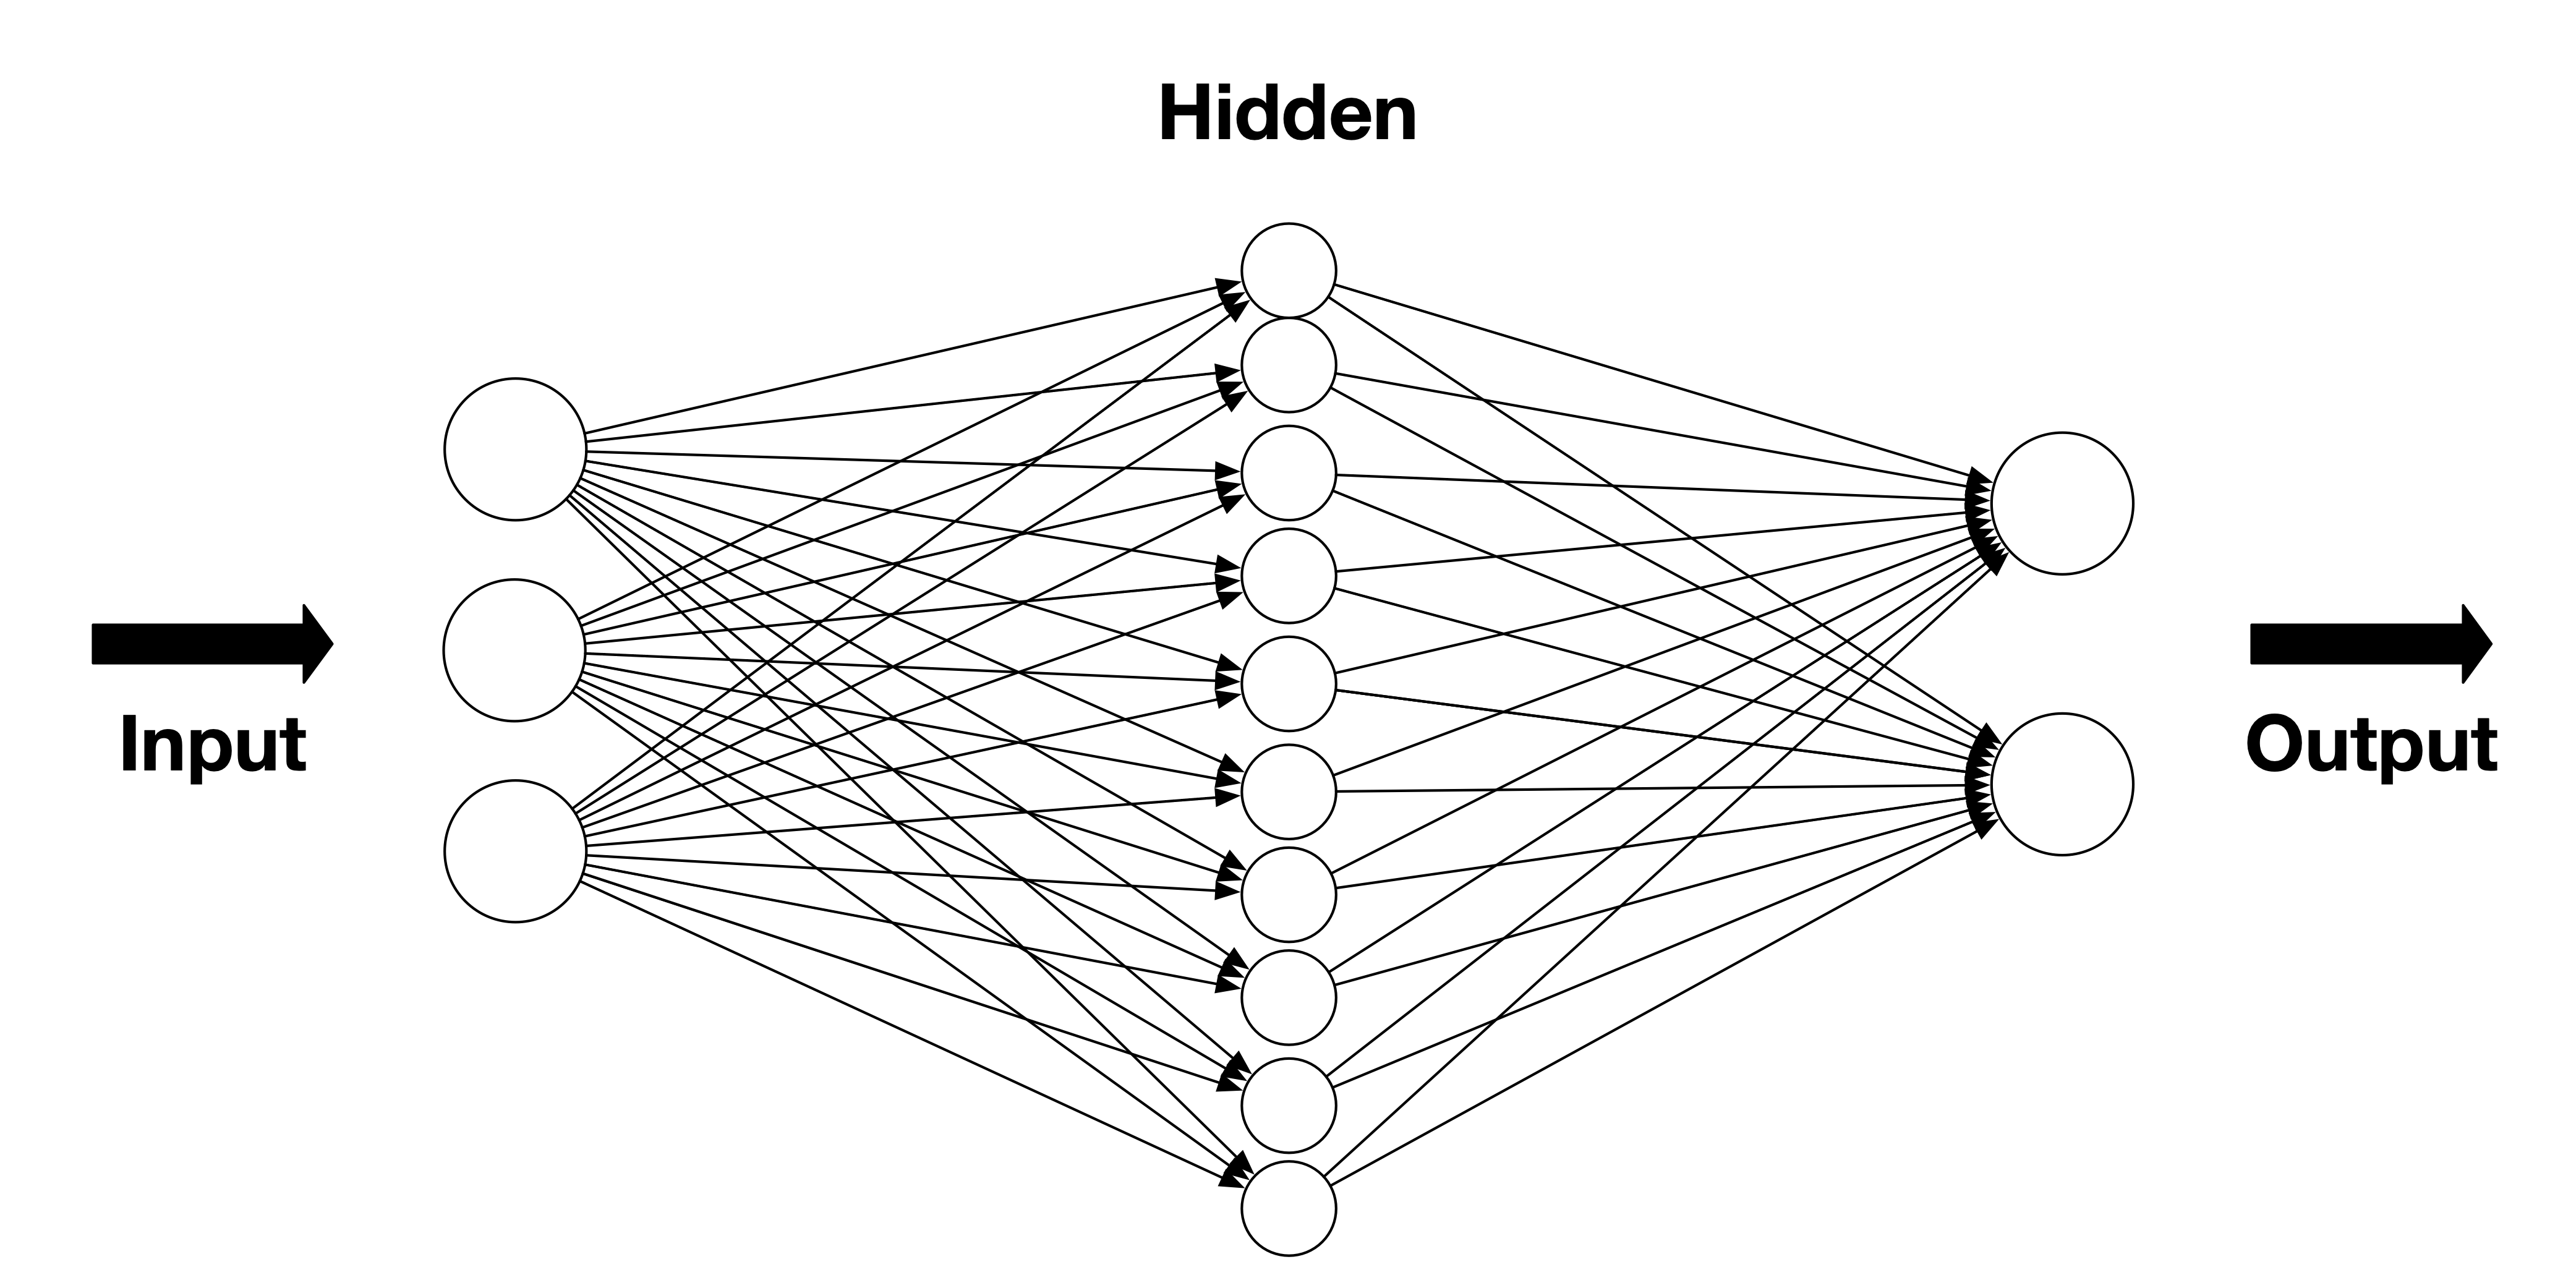
\includegraphics[width=\textwidth,keepaspectratio=true]{fig_snn}
    \caption{Illustrative representation of a Shallow Neural Network}
    \label{fig:fig_snn}
\end{figure}

\subsection{Out of Vocabulary Problem}
\label{nlp:oov}
A common issue in \gls{we} is related to the vocabulary itself when words are unknown, called the \gls{oov} issue. The issue occurs when post-training the model is requested to provide a vector representation that it never seen before. A solution could be to handle the exception by forwarding it to a default or pre-defined error vectors such as a series of zeros. We could approach the problem sophisticatedly, by defining on-the-fly \gls{oov} words with at a high learning rate as the sum of word-vectors contextualizing the \gls{oov}  \autocite{paper:journals/corr/HerbelotB17}. Another solution would be to fallback to \ref{nlp:ce} by either training a model to compositional map characters to words \autocite{paper:journals/corr/PinterGE17}, or using \gls{ce} as a whole instead of \gls{we} \ref{nlp:ce}.

\section{Character Embeddings}
\label{nlp:ce}
Additionally to \gls{we} similar abilities to capture semantics and syntactic relations, \gls{ce} handles by design \gls{oov} issues \ref{nlp:oov}, which is common for rich vocabularies languages. Instead of using words as vocabulary, \gls{ce} uses individual characters and semantics embeds words using the characters compositionally, which avoids word segmentation and makes it useful for language such as Chinese \autocite{paper:conf/ijcai/ChenXLSL15}. Moreover, \gls{ce} can also perform complementary \gls{nlp} tasks such as \gls{pos-tag} \autocite{paper:conf/icml/SantosZ14}, \gls{ner} \autocite{paper:ma-etal-2016-label}, Sentiment Analysis \autocite{paper:2017HaoYetal} and \gls{lm} \autocite{paper:journals/corr/KimJSR15}. As it is at the time of writing, \textit{FastText} based on the a morphologically-rich skip-gram approach \autocite{paper:journals/corr/BojanowskiGJM16} as been popularilized due to its ability to be scalabely trained on large corpora fast, and effectively. 


\label{nlp-lm}
Beyond complex semantics and syntaxes provided by \gls{we} \ref{nlp:we} and \gls{ce} \ref{nlp:ce}, \glspl{lm} handles \gls{cwe} by additionally capturing the polysemy across multiple contexts. Indeed, it was discovered that a distributed semantic, such as \gls{we} and \gls{ce} are not sufficient to infer context within the embeddings \autocite{paper:journals/corr/LucyG17}. A solution is to combine overall word representations from \gls{we} with \textit{ELMo} \autocite{paper:journals/corr/abs-1802-05365}, as its authors suggest, a \gls{bilm} able to build deep contextual word embeddings by handling multiple word representations. As mentioned in the study, handling polymesy is just one of the \glspl{lm} features as they are theoritized to capture meaningful \gls{nl} traits used in \gls{nlu} and \gls{nlg}. To increase the \gls{lm} quality, defined by language syntactic and semantical complexities captured, \gls{ul} on large corpora is popularly used, as no labeled data is required.


\section{Transformers}
\label{nlp:transformers}
The year 2017 has been a turnover in \gls{nlp} \autocite{paper:journals/corr/VaswaniSPUJGKP17}, transformers are since then defining the \gls{sota} for multiple \gls{nlp} tasks mainly due to its parallelized attention \ref{nlp:attention} architecture. Large multi-directional pre-trained \gls{lm} such as \gls{gpt2} or the \gls{bert} family are, additionally to their ability to capture features at sentence level, out-performing by a large margin previously mentioned \gls{nlp} technics at tasks such as \gls{qa} by performing \gls{model-ft}, an adaptation of the very popular Transfer Learning feature from computer vision. Making those new \gls{lm} currently trendy among \gls{nlp} researchers and engineers.

\begin{figure}
    \centering
    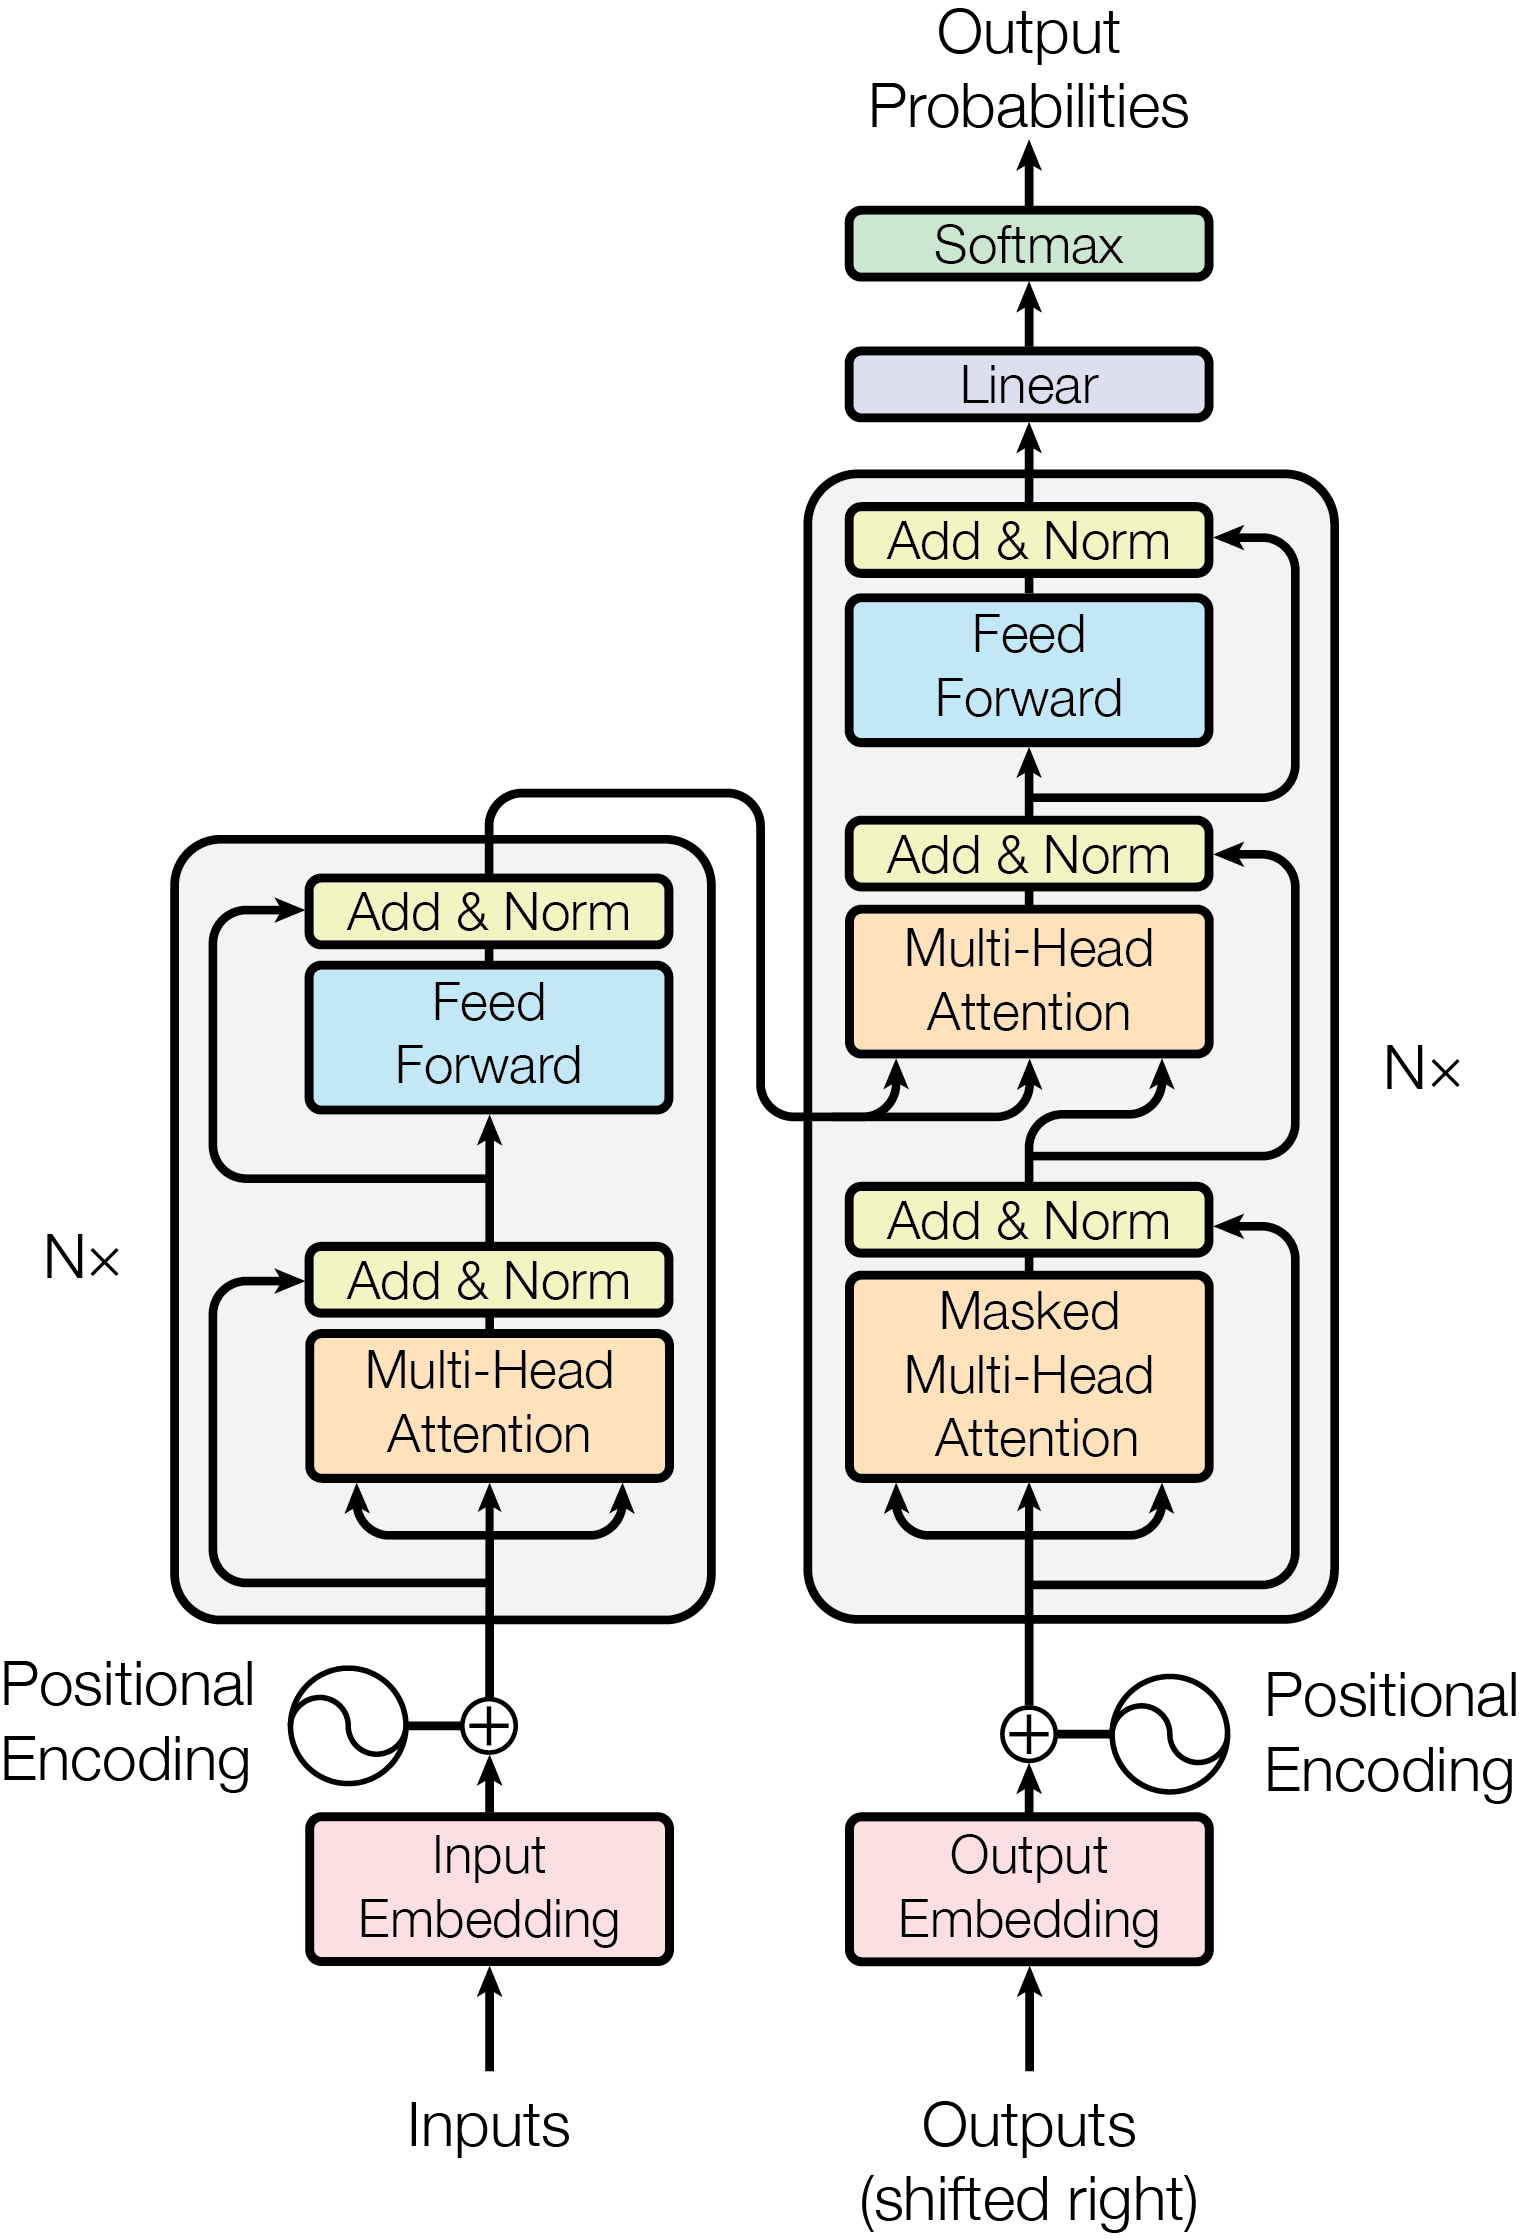
\includegraphics[width=\textwidth/2,keepaspectratio=true]{fig_external_transformer_1}
    \caption{Represents the Transformer architecture. Figure 1 from \autocite{paper:journals/corr/VaswaniSPUJGKP17}}
    \label{fig:fig_external_transformer_1}
\end{figure}

\subsection{Attention Mechanism}
\label{nlp:attention}
Introduced in 2014, The Attention Mechanism \autocite{paper:bahdanau2014neural} solved the problem raised by tasks such as text summarization, machine translation, or sentiment analysis, where the input is often too rich to perform a selective encoding. Originally, the last hidden state of the decoder is used by a multi-layer perceptron to define the attention from an input hidden state. The mechanism even got adapted from \gls{nlp} to Computer Vision and shown its ability to replace \gls{cnn} with \gls{sota} results \autocite{paper:journals/corr/abs-1906-05909}.

\begin{figure}
    \centering
    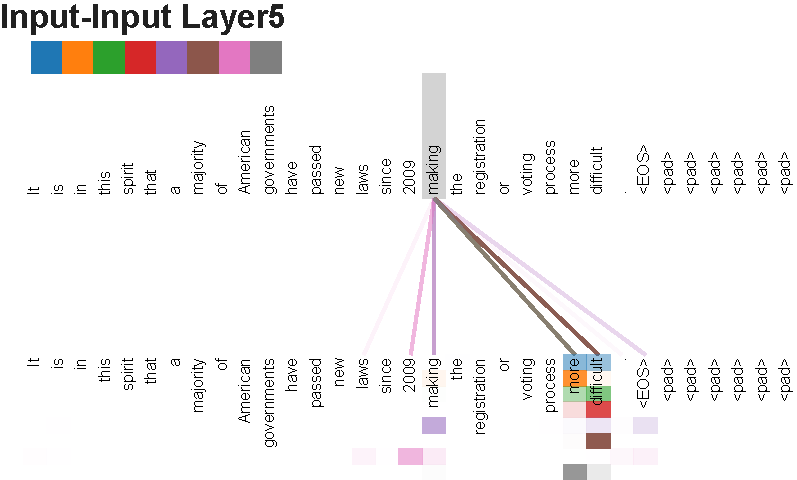
\includegraphics[width=\textwidth,keepaspectratio=true]{fig_external_transformer_3}
    \caption{Illustrates the attention mechanism for long-distance dependencies handled via multiple attention heads used in transformers. Figure 3 from \autocite{paper:journals/corr/VaswaniSPUJGKP17}}
    \label{fig:fig_external_transformer_3}
\end{figure}

\subsection{The architecture}
Even if Transformers, Figure \ref{fig:fig_external_transformer_1}, are using a \gls{seq2seq} approach similar to \gls{enc-dec}, which reminds of \gls{rnn} and \gls{cnn}, the overall architecture focuses on the attention mechanism to capture the relation between the input and the output, making it well parallelizable and less time consuming during training with its multi-attention heads approach. Multi-heads, Figure \ref{fig:fig_external_transformer_2_1}, uses sets of queries Q, keys K and values V to perform attention with dot-products, Figure \ref{fig:fig_external_transformer_2_2}. In other words, the multi-head attention mechanism builds a multi-dimensional matrix representing each word vectors the attention relatives to all word vectors in a predefined window, such as a sentence, then computes the overall attention for each word vectors. In addition to the attention centric mechanism, transformers are also using proven \gls{dl} techniques such as layer normalization, dropouts, and positional encodings.

\begin{figure}
	%\hfill
	%\centering
	\begin{subfigure}{.5\textwidth}
		\centering
		%
\includegraphics[width=.4\linewidth]{image1}
		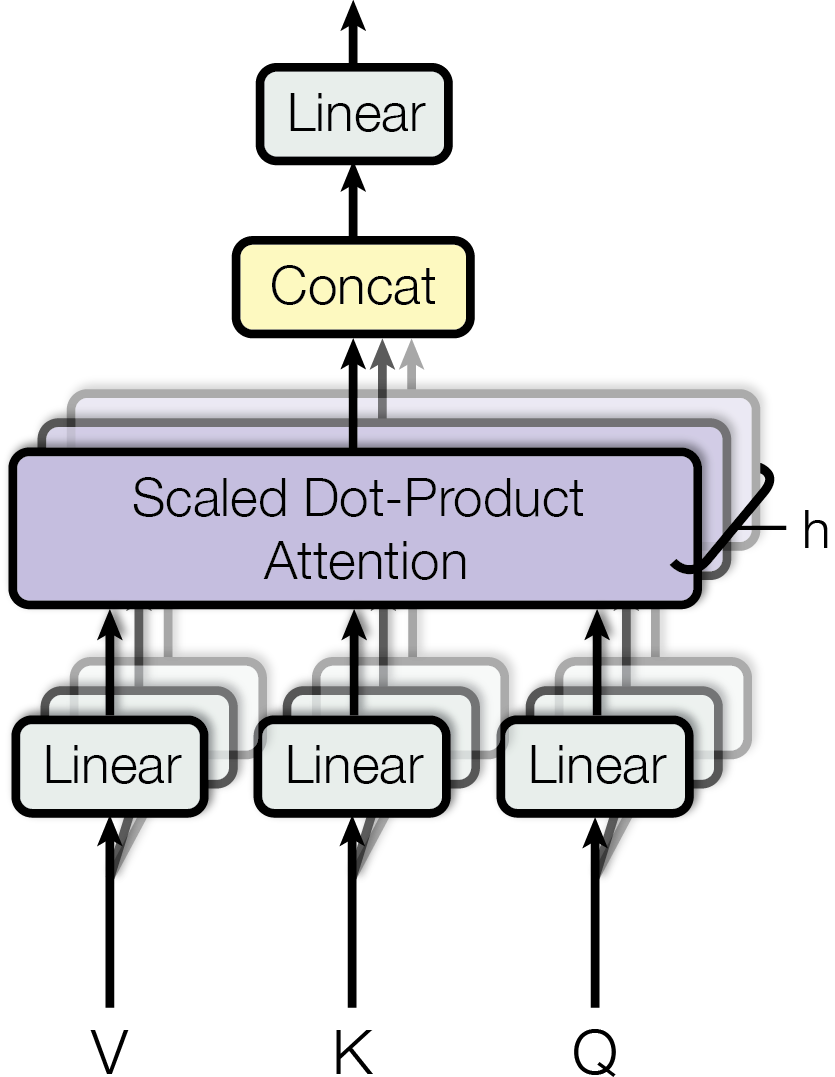
\includegraphics[width=\linewidth, height=1.2\linewidth, keepaspectratio=true]{fig_external_transformer_2_1}
		\caption{Multi-Head Attention mechanism.}
		\label{fig:fig_external_transformer_2_1}
	\end{subfigure}
	\hfill
	\begin{subfigure}{.5\textwidth}
		\centering
		%
\includegraphics[width=.4\linewidth]{image1}
		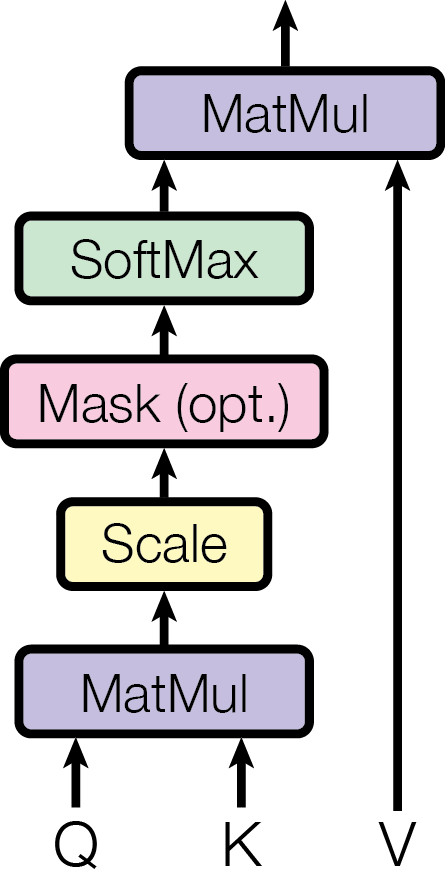
\includegraphics[width=1\linewidth, height=1.2\linewidth, keepaspectratio=true]{fig_external_transformer_2_2}
    	\caption{Scaled Dot-Product Attention used by the Multi-Heads Attention \ref{fig:fig_external_transformer_2_1}}
    	\label{fig:fig_external_transformer_2_2}
	\end{subfigure}
	%\hfill
	\caption{Multi-head attention anatomy extracted from Figure 2 of \textit{Attention is All you Need} \autocite{paper:journals/corr/VaswaniSPUJGKP17}}
	\label{fig:fig_external_transformer_2}
\end{figure}


\section{Honorable Mentions}
Even if Transformers have deprecated \gls{cnn} and \gls{rnn} in \gls{nlp} by solving their main bottleneck implying the sequential processing during encoding with the Attention Mechanism \ref{nlp:attention}. We still wanted to mention them as those techniques have defined baselines at multiple \gls{nlp} tasks for many years.

\subsection{Convolutional Neural Networks}
Commonly used in sentence modeling thanks to their good ability at mining semantics; however, their models are relatively heavy for the task performed. Additionally, they do not perform well on large windows, resulting in bad context handling for long-distance spread information and order tracking. In the field of \gls{qa}, interesting approach as been researched, such as Multi-Column \gls{cnn} \autocite{paper:Dong2015} able to treat multiple aspects of questions by building compatible representations with Wikidata's ancestor \textit{Freebase} \autocite{paper:bollacker2008}. In 2016, one of the final promising \gls{cnn} approach was introduced for \gls{qa} with a model able to handle relational information by word matching question and answer pairs \autocite{paper:Severyn2016}.

\subsection{Recurrent Neural Networks}
 By design and compared to \gls{cnn}, \glspl{rnn} try to take advantage of their ability to remember previous computations. However, it appears that no clear performance winner at \gls{nlp} tasks demarks \gls{rnn} from \gls{cnn} \autocite{paper:Yin2017}; indeed, their parallel performances depends on the global semantics and the task itself. Similarly to \gls{cnn}, \gls{rnn} is broadly used for \gls{nlp} tasks such as Language Modeling, Machine Translation, and Word/Sentence Classification.

\subsection{Memory Networks}
Also named MemNet \autocite{paper:Weston2015MemoryN}, the technique is still actively researched in the field of \gls{nlp} as it provides an intuitive approach to attention by using \gls{mh} \autocite{paper:journals/corr/TangQL16}, and sets the technique as an interesting competitor to Transformers \ref{nlp:transformers}. As the \gls{attention} \ref{nlp:attention} builds sets of hidden vectors with its encoder, \glspl{mn} uses the hidden vectors as internal memory instead of feeding them to a decoder for token generation. Further in the \glspl{transformer} competition, \glspl{mn} can be applied to similar \gls{nlp} tasks such as \gls{qa} \autocite{paper:journals/corr/KumarISBEPOGS15} by extending the (representation, attention, answer) tuples to \textit{(Memory, Question, Answer)} tuples. The Figure \ref{fig:fig_external_memnet} presents a \gls{qa} architecture using a knowledge source, for instance a knowledge base, as the initial Key-Value Memories provider, \glspl{spo}. 

\begin{figure}
    \centering
    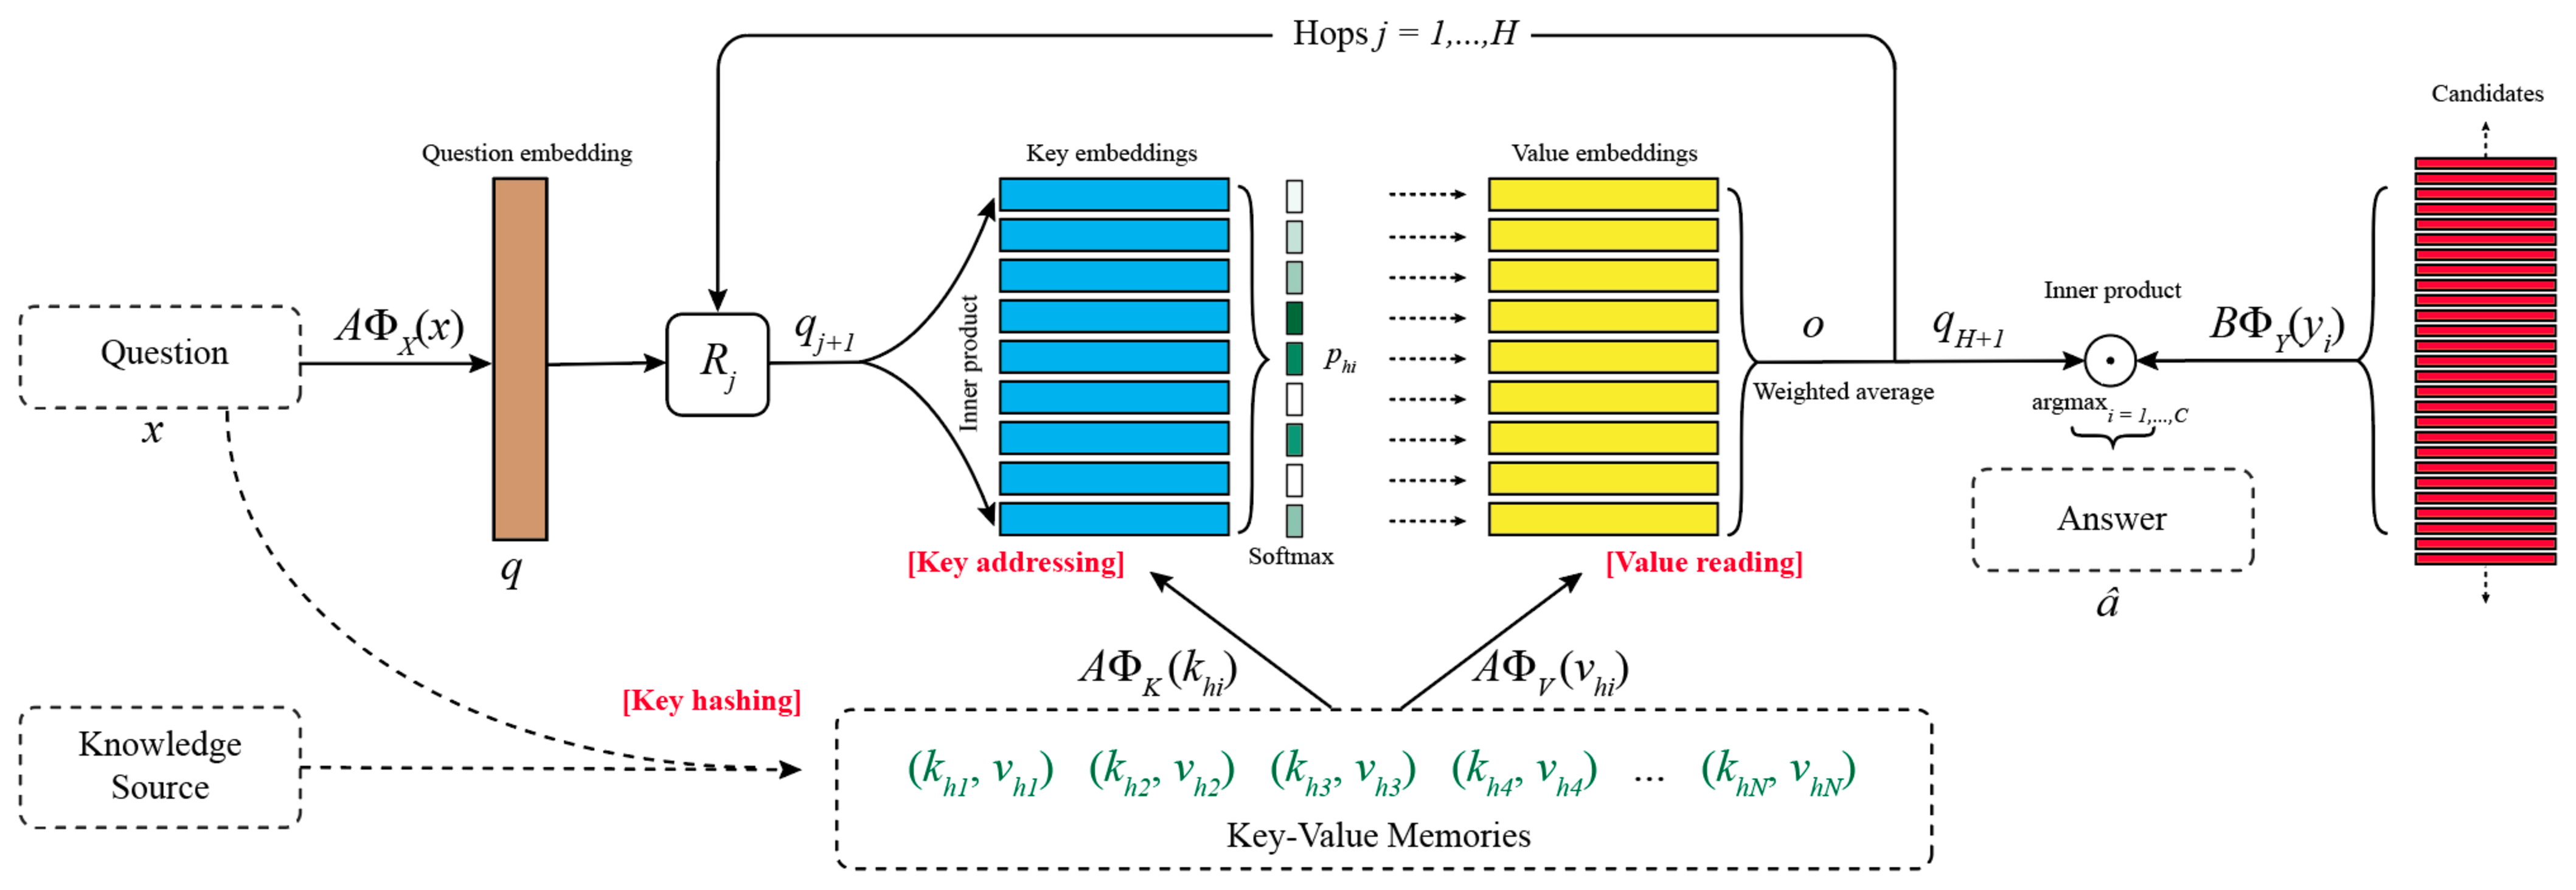
\includegraphics[width=\textwidth,keepaspectratio=true]{fig_external_memnet}
    \caption{Illustrates a Key-Value Memory Network model used in \gls{qa}. Figure 1 from \autocite{paper:journals/corr/MillerFDKBW16}}
    \label{fig:fig_external_memnet}
\end{figure}


%\section{Common Natural Language Processing Features}
%Most of the following technics have been introduced to \gls{nlp} by the \glsfirst{ir} field. Indeed

%\subsection{Deep Learning}
%\todo{What are the problems such as bias, and how it can accumulate? Used to predict the next step. Various techniques, such as generative, recursive, etc.}

%\subsection{Unsupervised Deep Learning}
%\todo{How and when unsupervised training is helpful for NLP. What are the techniques. Talk about fine tuning and re-training.}
